\section{Dataset and Simulated Events}
\label{sec:analysis:dataset}


\subsection{Data}
\label{sec:analysis:dataset:data}

In this analysis, data is selected based on the presence of at least one muon or one electron. The single muon dataset requires that events contain at least one muon with $\pt > 25\GeV$ and passing the loose track isolation criterion, $\rm Iso_{track} < 0.1$. The single electron dataset requires that there be at least one electron satisfying the requirement that $\pt > 30\GeV$ and that it passes the tight identification requirements as defined by the EGamma POG.  The specific dataset names and the associated integrated luminosities are listed in Table~\ref{tab:analysis:dataset:data2016}.


    % \small
    \begin{tabular}{l c c}
        \hline
        Sample                                              & Run ranges    & $\int L (\fbinv)$ \\
        \hline
        \texttt{SingleMuon/Run2016B-03Feb2017\_ver2-v2}     & 272007-275376 & 5.33                \\
        \texttt{SingleMuon/Run2016C-03Feb2017-v2}           & 275657-276283 & 2.4                 \\
        \texttt{SingleMuon/Run2016D-03Feb2017-v2}           & 276315-276811 & 4.26                \\
        \texttt{SingleMuon/Run2016E-03Feb2017-v2}           & 276831-277420 & 4.1                 \\
        \texttt{SingleMuon/Run2016F-03Feb2017-v2}           & 277772-278808 & 3.2                 \\
        \texttt{SingleMuon/Run2016G-03Feb2017-v2}           & 278820-280385 & 7.8                 \\
        \texttt{SingleMuon/Run2016H-03Feb2017\_ver*-v1}     & 281613-284044 & 9.2                 \\
        \hline
        \texttt{SingleElectron/Run2016B-03Feb2017\_ver2-v2} & 272007-275376 & 5.33                  \\
        \texttt{SingleElectron/Run2016C-03Feb2017-v2}       & 275657-276283 & 2.4                   \\
        \texttt{SingleElectron/Run2016D-03Feb2017-v2}       & 276315-276811 & 4.26                  \\
        \texttt{SingleElectron/Run2016E-03Feb2017-v2}       & 276831-277420 & 4.1                   \\
        \texttt{SingleElectron/Run2016F-03Feb2017-v2}       & 277772-278808 & 3.2                   \\
        \texttt{SingleElectron/Run2016G-03Feb2017-v2}       & 278820-280385 & 7.8                   \\
        \texttt{SingleElectron/Run2016H-03Feb2017\_ver*-v1} & 281613-284044 & 9.2                   \\
        \hline
    \end{tabular}



\noindent Run ranges where data quality is determined to be insufficient are filtered removed from the datset by applying a luminosity mask. The following file is provided in JSON format from the CMS PPD group:

\texttt{Cert\_271036-284044\_13TeV\_23Sep2016ReReco\_Collisions16\_JSON.txt}

\noindent The full dataset consists of 35.9\fbinv of integrated luminosity~\cite{cms:lumi2016:CMS-PAS-LUM-17-001}




\subsection{Simulated Dataset}
\label{sec:analysis:dataset:simulation}

Simulated datasets are used for modelling the major SM processes, including SM diboson, $\PW/\PZ/\PGg$ associated with jets, single-top and \ttbar. The background from multijet QCD is estimated by a data-driven approach discussed in section~\ref{sec:analysis:background} The simulated samples used in modelling the background and signal are shown in table~\ref{tab:analysis:dataset:mc2016}.  The production of the samples was carried during the Summer 2016 campaingn and the production of the mini Analysis Oriented Data format (miniAOD) was done using CMSSW release \texttt{8\_0\_26\_patch2}. The same release was used for processing both the data and the simulated samples. Lepton universality is assumed for the simulated datasets, namely $ \BWl = 10.8\%$. To account for the deviation from the data, some reweightings of the simulated dataset are applied, commonly including reweightings for pile-up, top \pt, \WW \pt and \PZ \pt.

\begin{table}[ht]
    \centering
    \setlength{\tabcolsep}{2em}
    \renewcommand{\arraystretch}{1.1}
    \caption{Simulated MC samples.} \label{tab:dat:mc2016}
    % \small
    \begin{tabular}{l l c}
        \hline
        Process                                           & Generator         & $\sigma \times \text{BR} (pb)$ \\
        \hline
        $t\bar{t}$                                        & \POWHEG+\PYTHIA     & 831.76                        \\
        $t\bar{t}$  (leptonic)                            & \POWHEG+\PYTHIA     & 87.32                          \\
        $t\bar{t}$  (semi-leptonic)                       & \POWHEG+\PYTHIA     & 364.35                         \\
        $tW/\bar{t}W$                                     & \POWHEG+\PYTHIA     & 35.6                           \\
        \hline
        Z+jets                                            &                  &                                \\
        \hspace*{1em} $10 < m_{\ell\ell} < 50$ GeV        & \MCATNLO+\PYTHIA   & 18610                          \\
        \hspace*{1em} $m_{\ell\ell} > 50 $GeV             & \MCATNLO+\PYTHIA   & 5765                           \\
        \hspace*{1em} $m_{\ell\ell} > 50, N_{j} = 0 $GeV  & \MCATNLO+\PYTHIA   & 4757                           \\
        \hspace*{1em} $m_{\ell\ell} > 50, N_{j} = 1 $GeV  & \MCATNLO+\PYTHIA   & 884.4                          \\
        \hspace*{1em} $m_{\ell\ell} > 50, N_{j} = 2 $GeV  & \MCATNLO+\PYTHIA   & 338.9                          \\
        \hline
        W + 1 jet                                         & \MADGRAPH+\PYTHIA  & 11486.5                        \\
        W + 2 jet                                         & \MADGRAPH+\PYTHIA  & 3775.2                         \\
        W + 3 jet                                         & \MADGRAPH+\PYTHIA  & 1139.8                         \\
        W + 4 jet                                         & \MADGRAPH+\PYTHIA  & 655.82                         \\
        \hline
        $qq\rightarrow WW \rightarrow 2\ell 2\nu$         & \POWHEG           & 12.13                          \\
        $gg\rightarrow WW \rightarrow 2\ell 2\nu$         & \POWHEG           & 0.588                          \\
        WZ $\rightarrow 3\ell \nu$                        & \POWHEG+\PYTHIA    & 5.29                           \\
        WZ $\rightarrow 2\ell 2q$                         & \MCATNLO+\PYTHIA   & 5.595                          \\
        ZZ $\rightarrow 2\ell 2\nu$                       & \POWHEG+\PYTHIA    & 0.564                          \\
        ZZ $\rightarrow 2\ell 2q$                         & \MCATNLO+\PYTHIA   & 3.22                           \\
        ZZ $\rightarrow 4\ell$                            & \MCATNLO+\PYTHIA   & 1.21                           \\
        \hline
    \end{tabular}

    
\end{table}







% \subsection{Standard Reweightings}

% % tau decay
% \subsubsection{$Br(\tau)$ Reweighting}

% The tau decay modes diverge slightly from the values listed in the PDG as can be seen in Table~\ref{tab:dat:tauDecayBr}. The MC events have been reweighted according to their gen-level tau decay mode to correct the tau decay in the simulation to the PDG experimental value. The impact of this on the branching fraction determination is estimated and included as a systematic uncertainty
% \begin{table}[ht]
    \centering
    \setlength{\tabcolsep}{2em}
    \renewcommand{\arraystretch}{1.5}
    % \small
    \begin{tabular}{l|cc}
        decay                                & simulation & PDG       \\
        \hline
        $e$                                  & 0.17728    & 0.1782(4) \\
        $\mu$                                & 0.17311    & 0.1739(4) \\
        $\pi^{\pm}$                          & 0.10768    & 0.1082(5) \\
        $\pi^{\pm}\pi^{0}$                   & 0.25374    & 0.2549(9) \\
        $\pi^{\pm}\pi^{0}\pi^{0}$            & 0.09247    & 0.0926(10) \\
        $\pi^{\pm}\pi^{\pm}\pi^{\mp}$        & 0.09257    & 0.0931(5) \\
        $\pi^{\pm}\pi^{\pm}\pi^{\mp}\pi^{0}$ & 0.04594    & 0.0462(5) \\
        5 prong                              & ?          & $9.9(4)\times 10^{-4}$ \\
    \end{tabular}
    \caption{Comparison of $\tau$ lepton branching fractions used in simulation of its decays and those listed in the PDG.} 
    \label{tab:dat:tauDecayBr}
\end{table}



% pu
\subsubsection{Pile-up Reweighting}
Differences between the pileup distribution used in simulation and data is corrected by reweighting the simulation according to the weights shown in figure~\ref{fig:analysis:dataset:pileup}. The weight is applied based on the number of pileup, including out-of-time pileup, per event.  This process can be validated by comparing the number of reconstructed primary vertices in data and simulation as shown in figure~\ref{fig:analysis:dataset:pileup} right. There is still a sizeable discrepancy between the distributions. This has been widely observed within CMS and no additional measures are taken to address this.


\begin{figure}[ht]
    \centering
    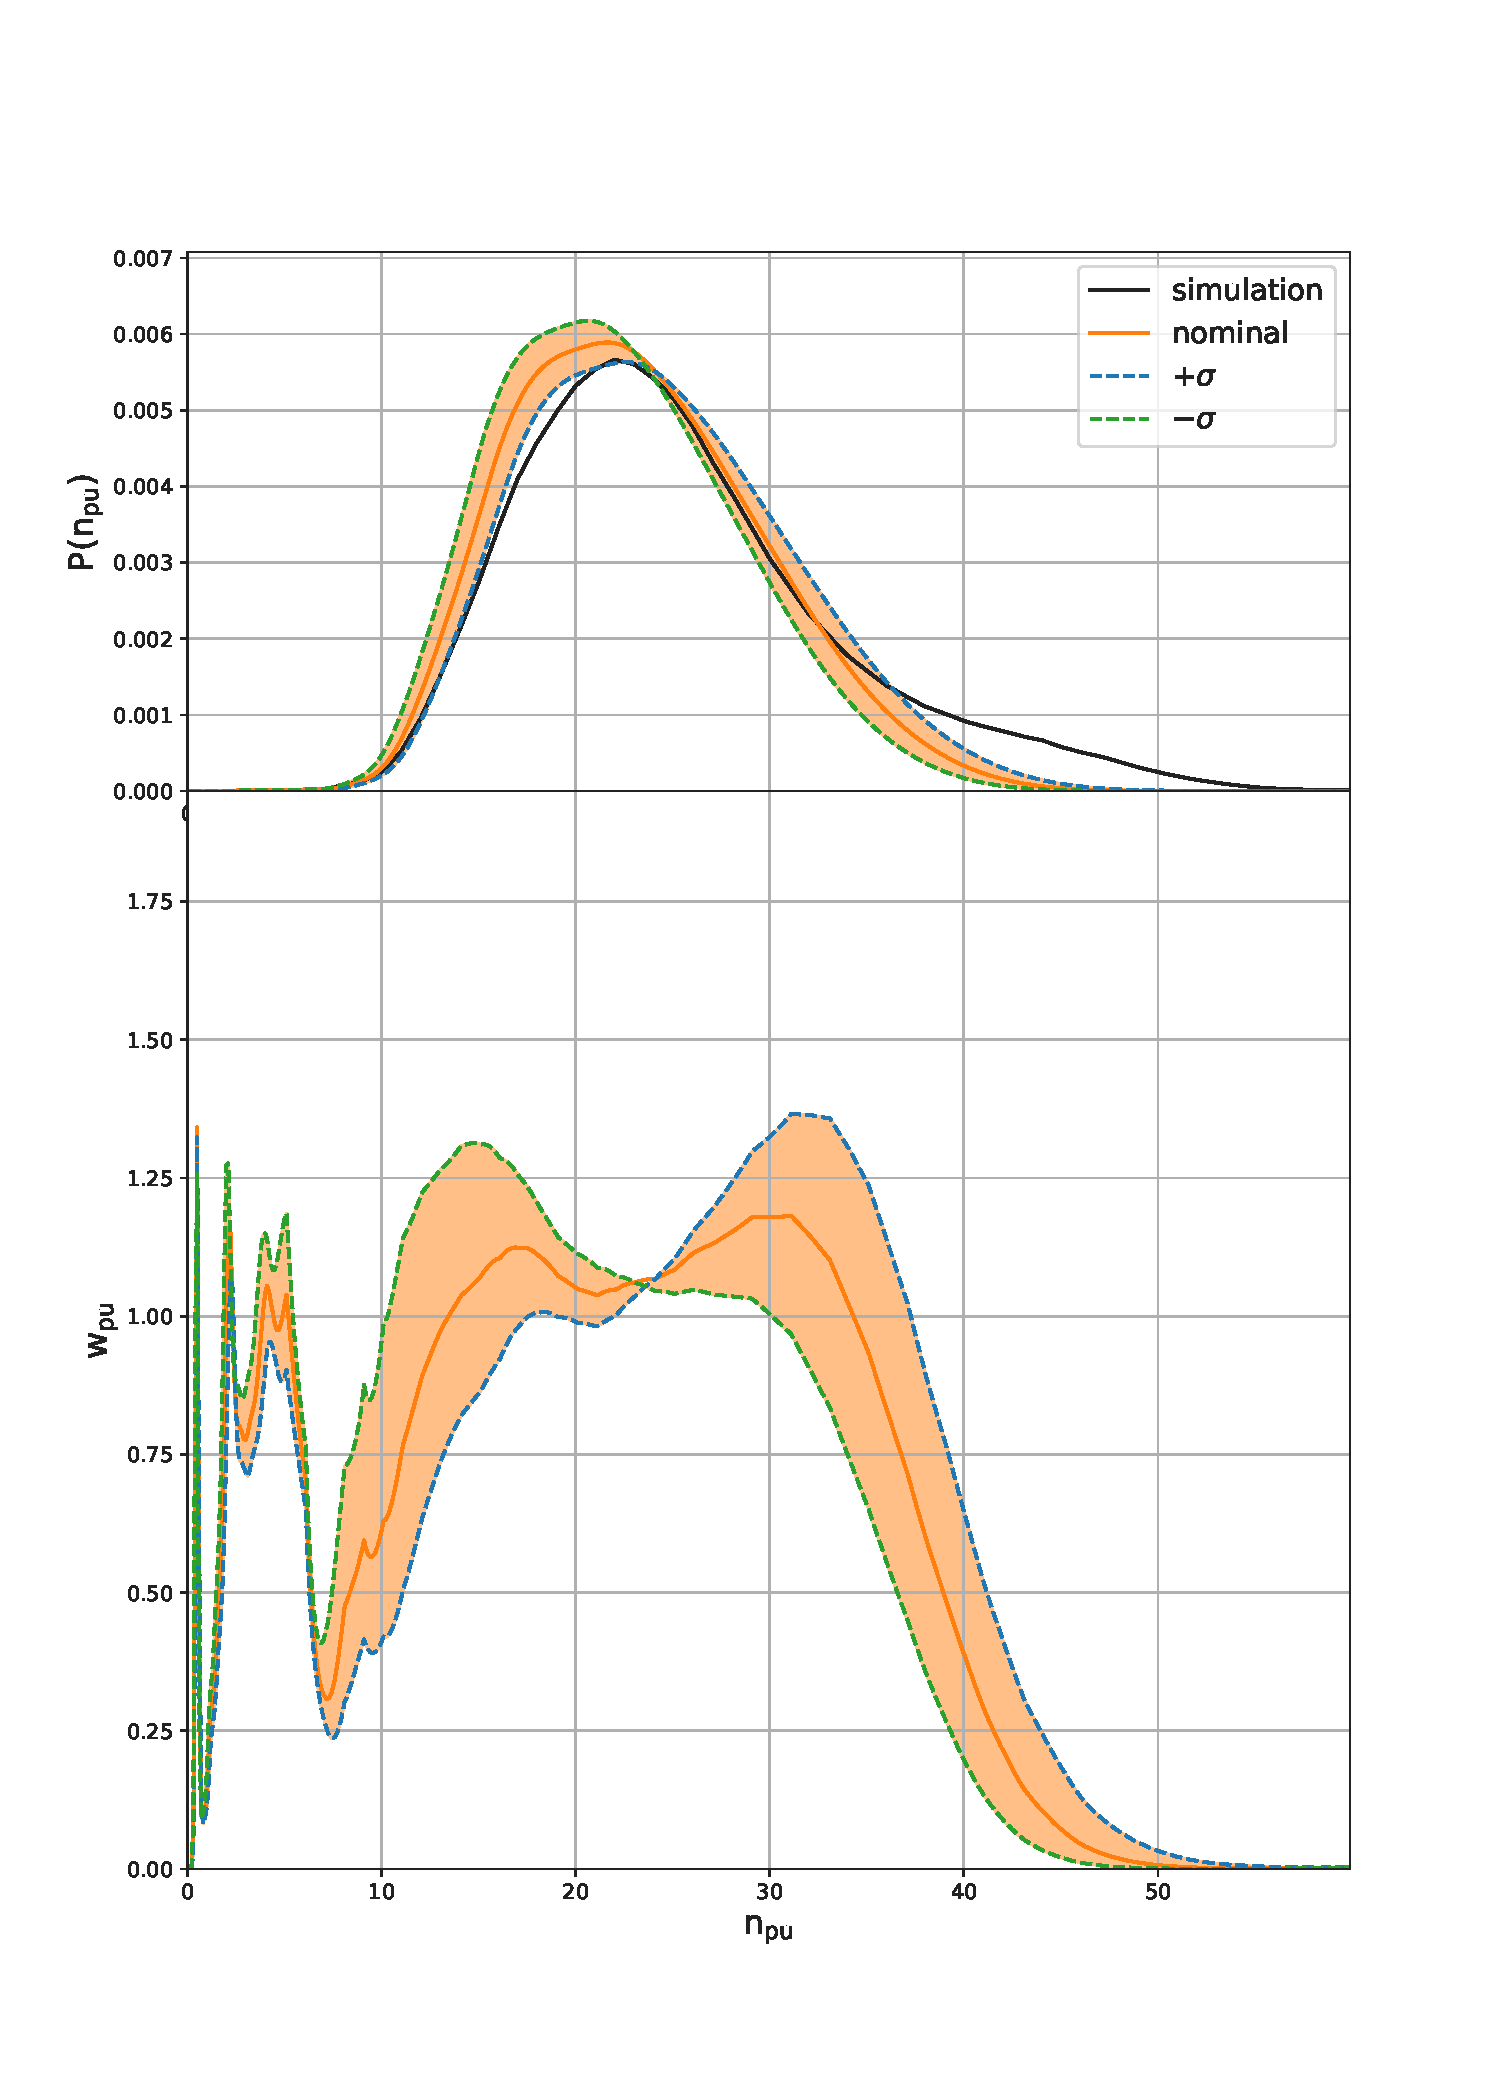
\includegraphics[height=0.42\textheight]{chapters/Analysis/sectionDataset/figures/pileup_systematics.pdf}
    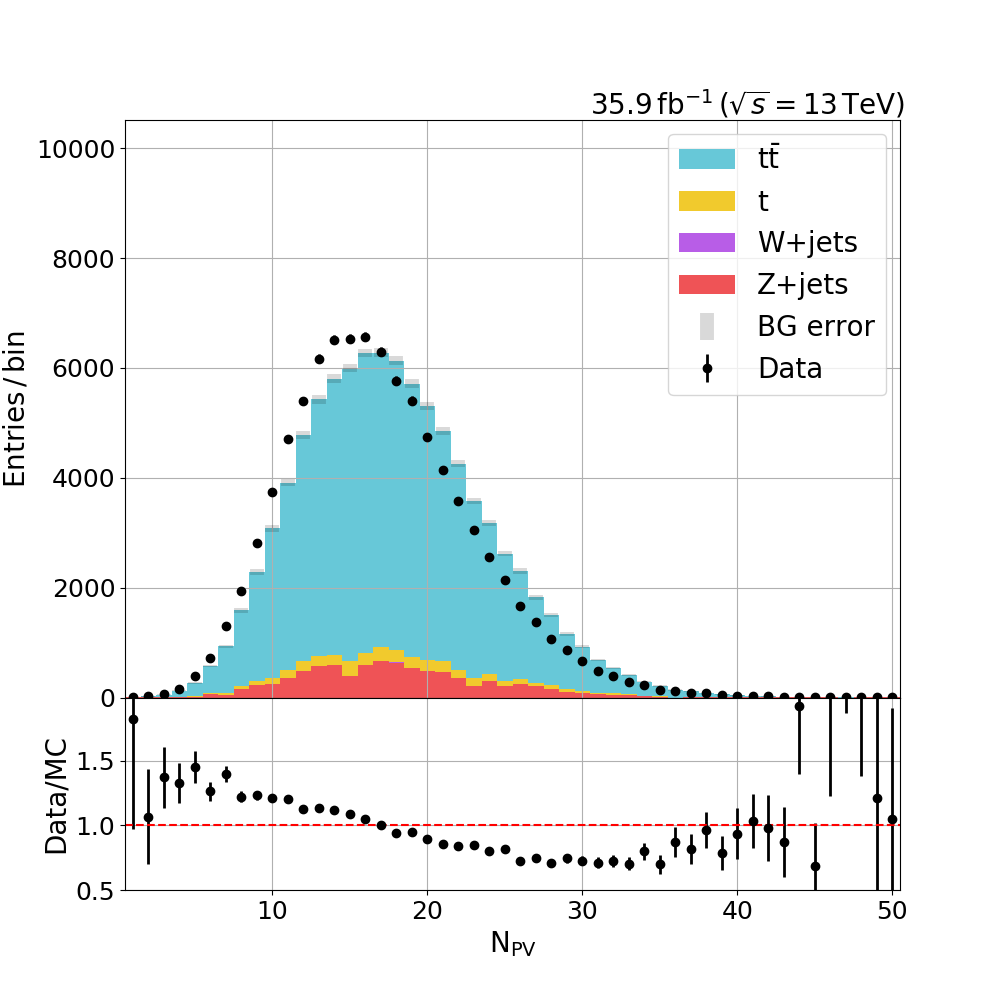
\includegraphics[height=0.42\textheight]{chapters/Analysis/sectionDataset/figures/n_pv}
    \caption{\emph{(left top)} Pileup distribution in data and simulation including the $\pm\sigma$ variation of the data pileup distributions. \emph{(left bottom)} The weights parameterized by number of simulated pileup resulting from taking the ratio of the pileup distribution in data and simulation. \emph{(right)} Comparison of primary vertex multiplicity between data and simulated datasets. }
    \label{fig:analysis:dataset:pileup}
\end{figure}


\FloatBarrier


%  top pt
\subsubsection{Top \pt Reweighting}

Additional corrections can be applied to the \ttbar sample to account for generator level mismodeling of the top quark \pt spectrum~\cite{CMS-PAS-TOP-16-011, CMS-PAS-TOP-16-008}.  This is done by identifying the parton-level top quarks, and calculating a scale factor from the equation,

\begin{equation*}
    SF_{\PQt}(\pt) = SF_{\PAQt}(\pt) = e^{0.0615-0.0005 \pt}.
\end{equation*}


\noindent The overall event weight is that is applied is $w = \sqrt{SF_{\PQt}SF_{\PAQt}}$.  For this analysis, we do not apply the weight, but instead use it as the systematical uncertainties associated with the top \pt correction.

\begin{figure}[ht]
    \centering
    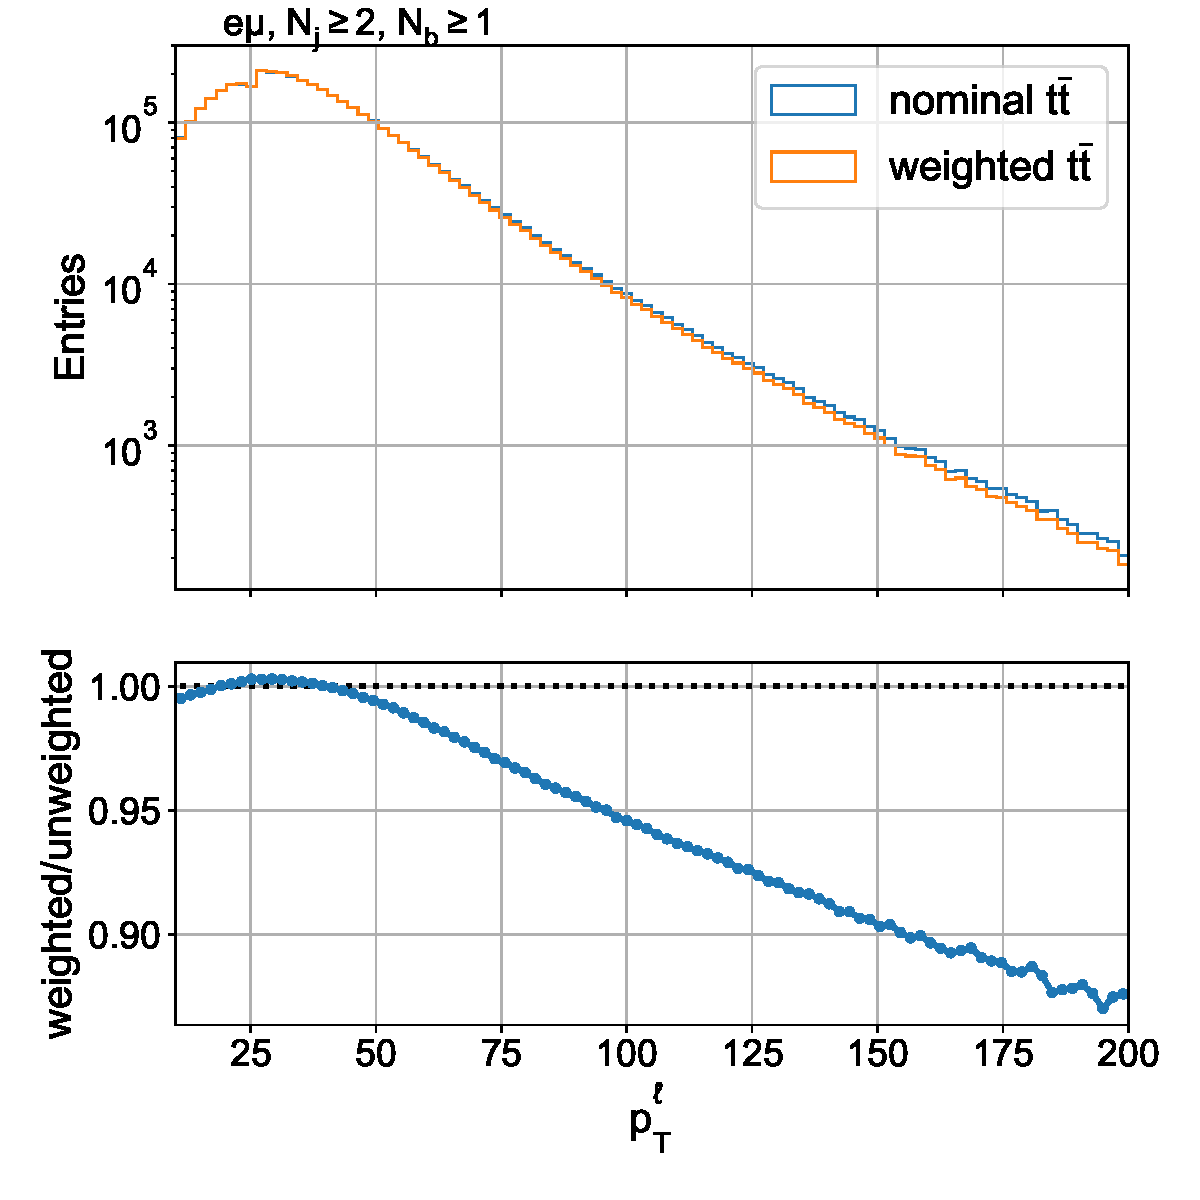
\includegraphics[width=0.55\textwidth]{chapters/Analysis/sectionDataset/figures/top_pt_weight}
    \caption{Comparison of the trailing lepton \pt distribution in $\cem$ events with at least two jets and at least one \PQb tag with top \pt weights applied and without the weights.}
    \label{fig:analysis:dataset:top_pt_weight}
\end{figure}


% ww pt
\subsubsection{\WW \pt Reweighting}
Estimation of the \WW process relies on the \POWHEG MC generator which is a NLO fixed order generator. Higher order corrections are therefore not directly included, but have been calculated separately~\cite{Meade:2014fca, Jaiswal:2014yba, Grazzini:2015wpa}.  The estimation of uncertainty is based on the description in AN-2017-273. As mentioned there, the theoretical uncertainty associated with the corrections have not been provided so they are estimated by varying the renormalization, factorization, and the matching scale of the \pt resummation technique. The weights and their systematic variations, as well as the effect on the lepton \pt spectrum in the \WW MC sample is shown in figure~\ref{fig:analysis:dataset:ww_weight}.

\begin{figure}[ht]
    \centering
    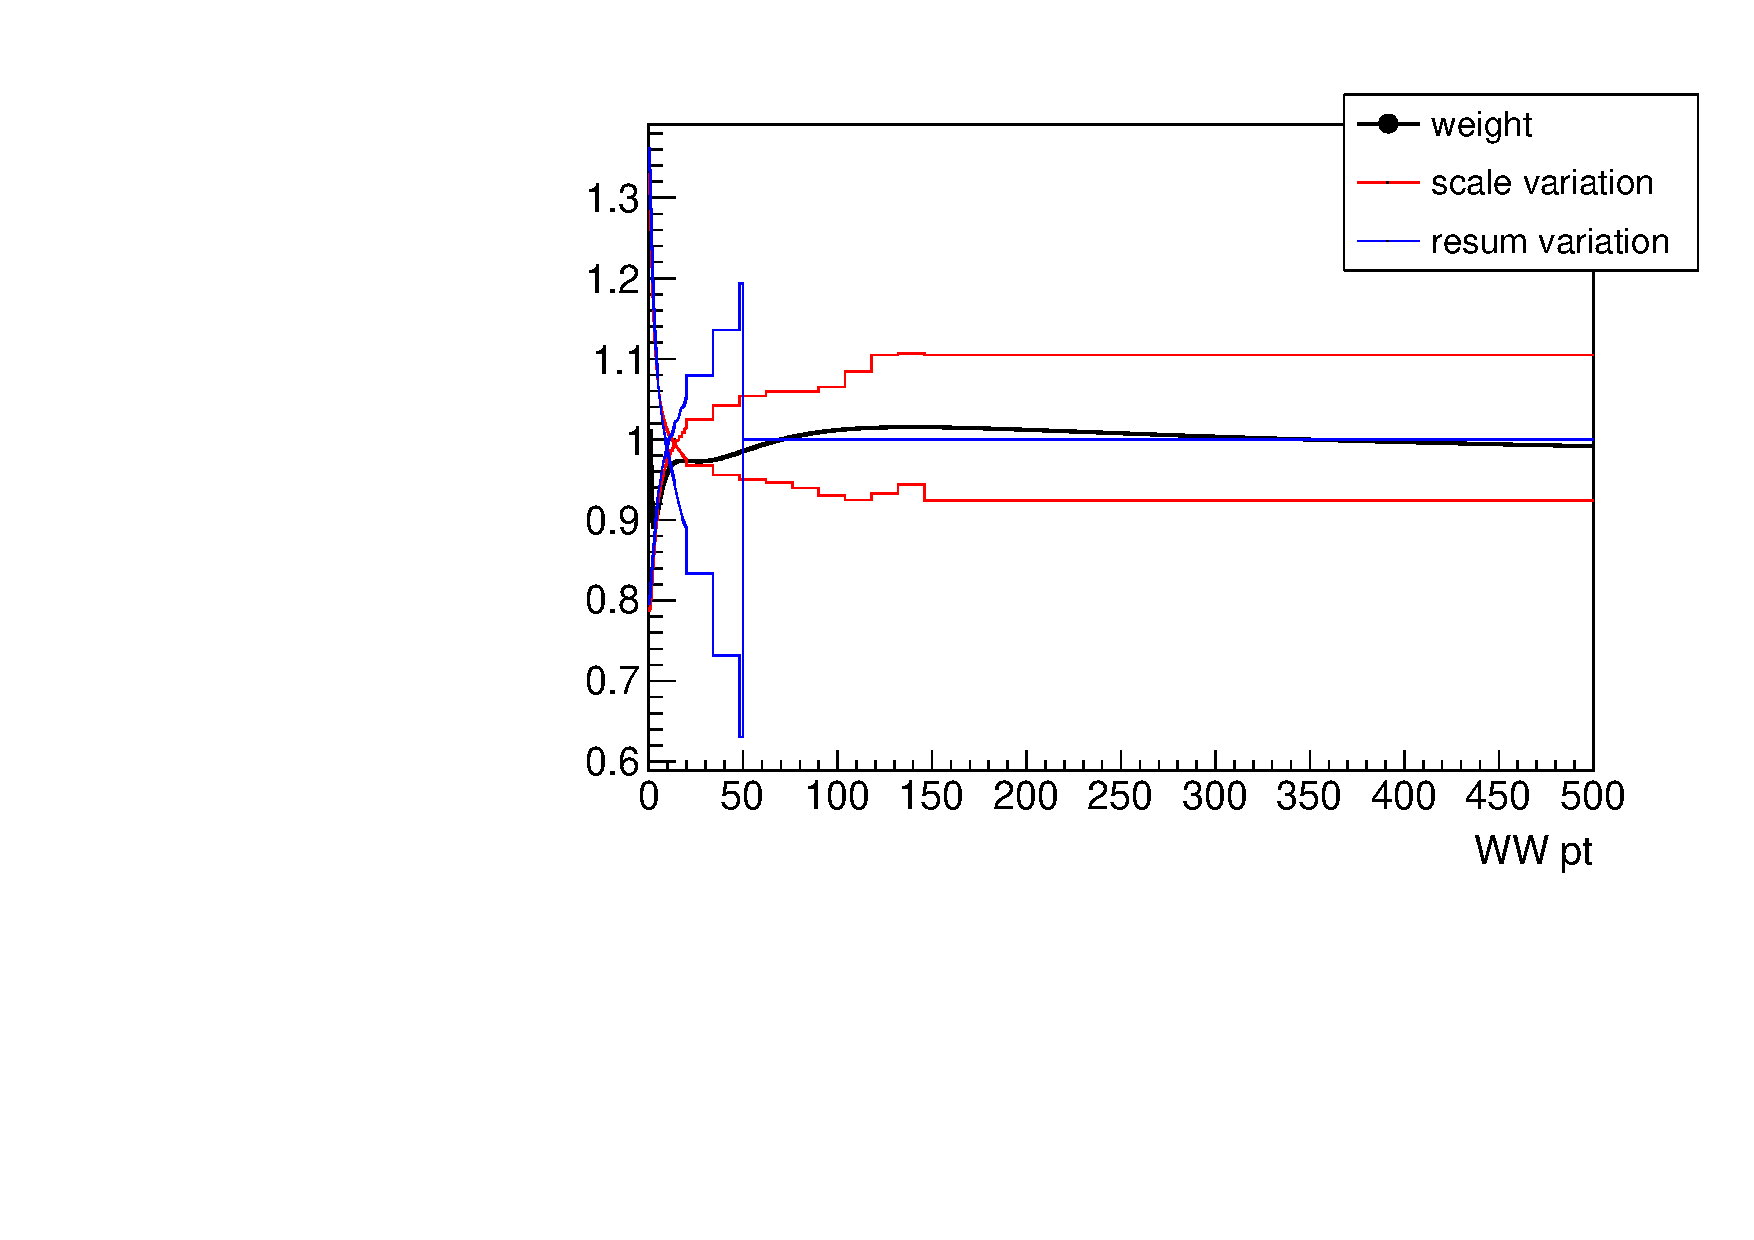
\includegraphics[width=0.5\textwidth]{chapters/Analysis/sectionDataset/figures/ww_pt_weight_variations}
    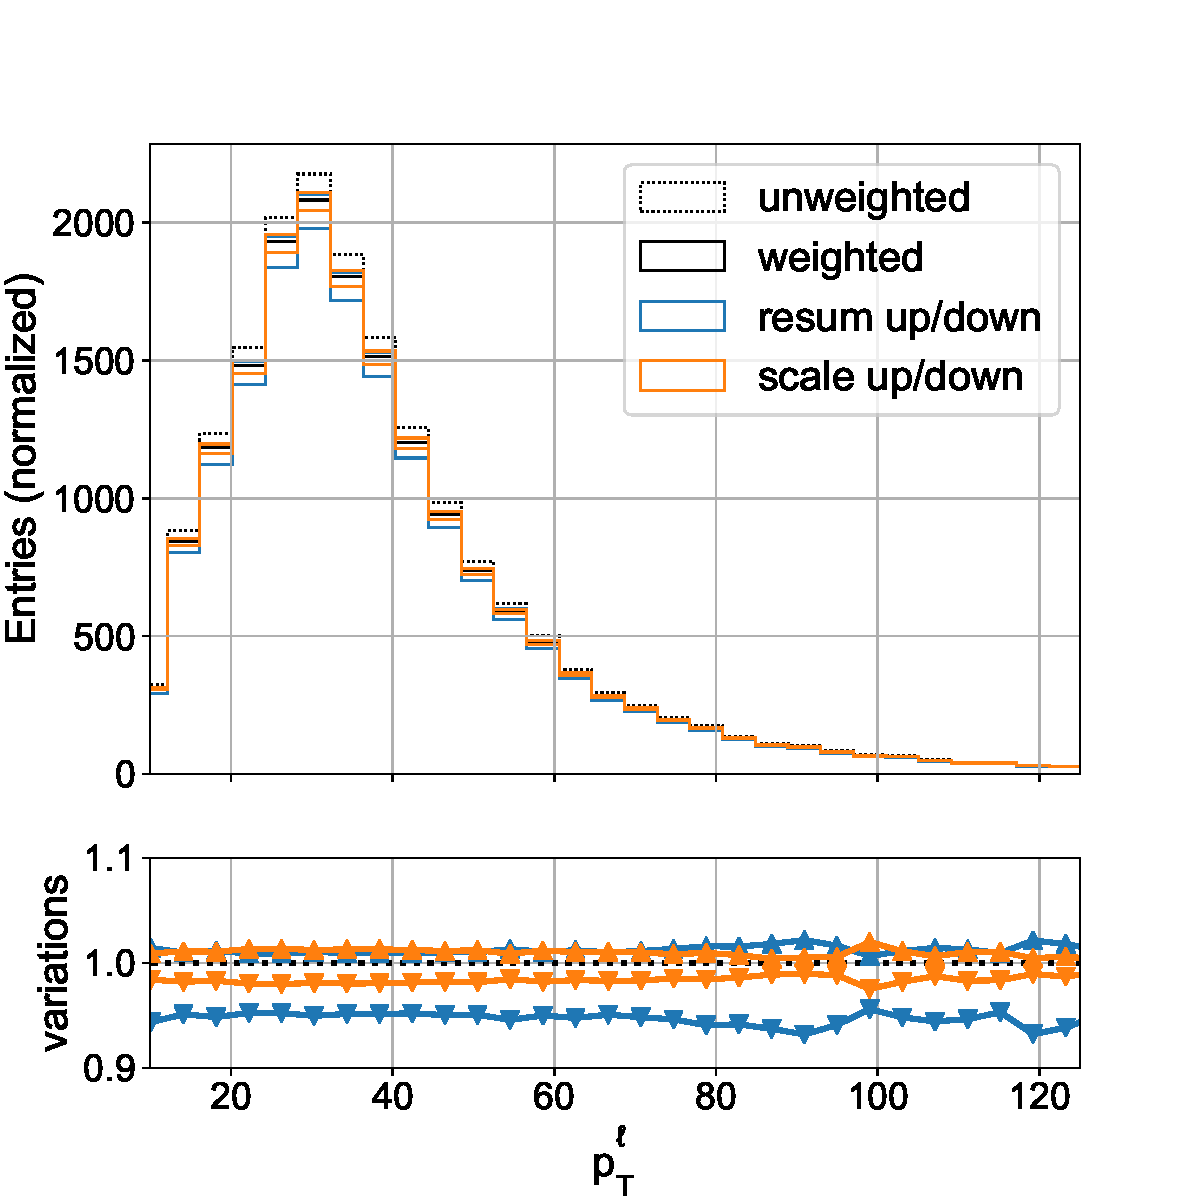
\includegraphics[width=0.38\textwidth]{chapters/Analysis/sectionDataset/figures/ww_pt_lepton_pt}
    \caption{\emph{(left)} Weights for the $\PQq \PQq \rightarrow \WW$ process as a function of the $\WW\,\pt$ and the two componnents of systematic variation.  \emph{(right)} Trailing lepton pt from the $\PQq \PQq\rightarrow \WW\rightarrow \cem\PGn\PGn$ simulated sample when there are no reconstructed jets.} 
    \label{fig:analysis:dataset:ww_weight}
\end{figure}



% z pt
\subsubsection{\PZ \pt Reweighting}
Based on differences between the observed and predicted \PZ \pt spectrums, weights are derived to correct the \pt spectrum in simulation. The derivation of the weights was done in the context of the $\PH \rightarrow \WW $ analysis and is described in AN-2017-082. This correction does not have an associated uncertainty.

\begin{figure}[ht]
    \centering
    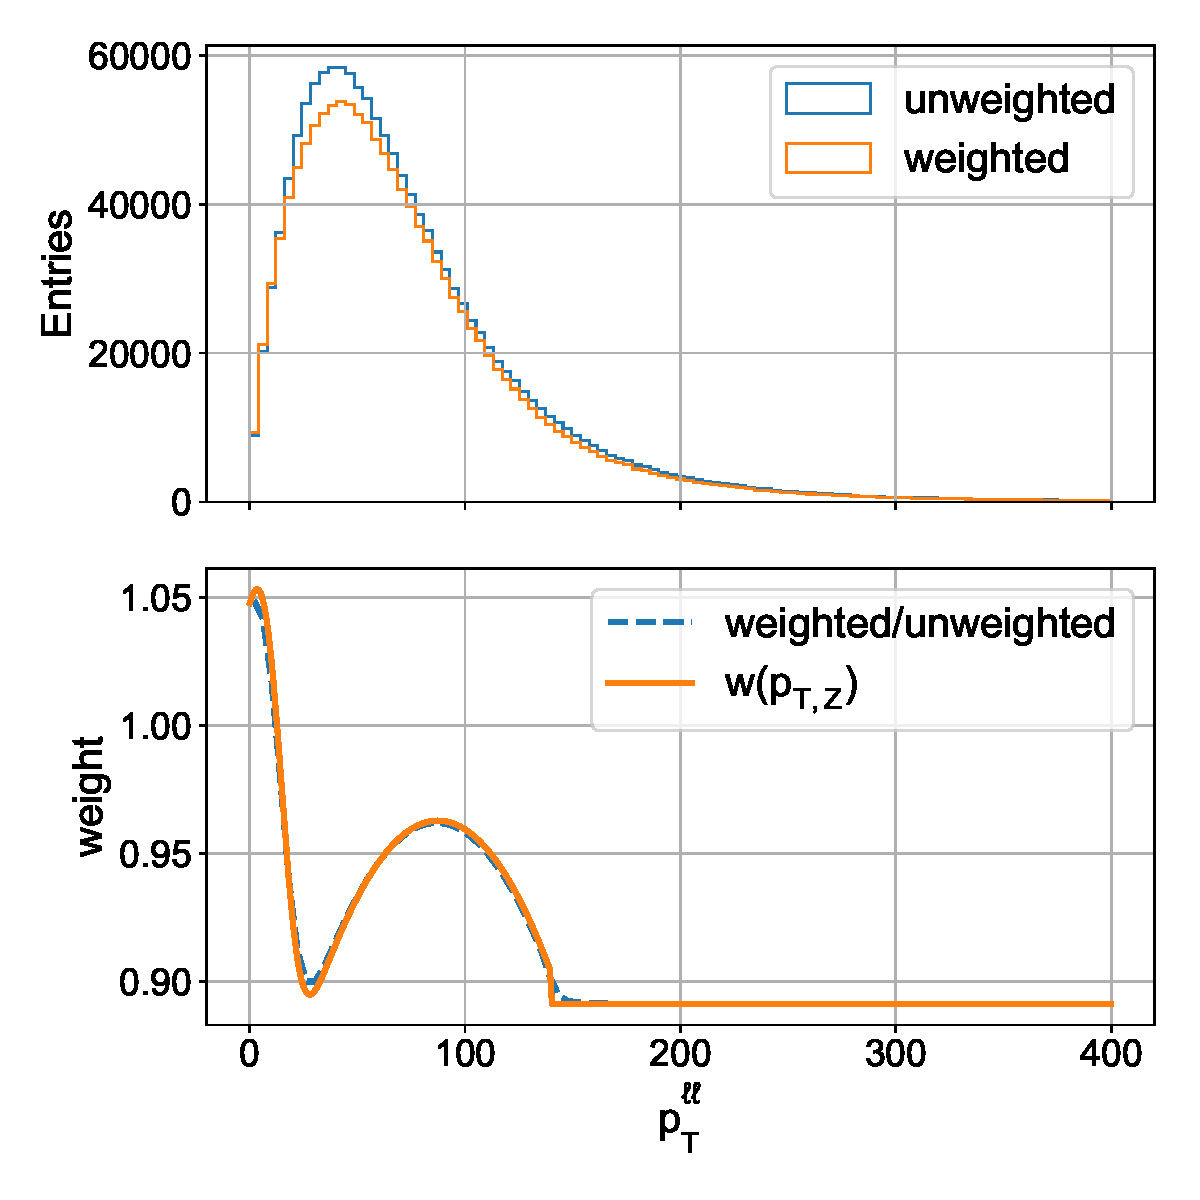
\includegraphics[width=0.55\textwidth]{chapters/Analysis/sectionDataset/figures/z_pt_weighting}
    \caption{\emph{(top)} Comparison of weighted and unweighted dilepton \pt spectrum for dimuon events with two jets and no \PQb tags. \emph{(bottom)} Comparison between ration of distributions in the top distribution and the analytical function for generating weights.}
    \label{fig:analysis:dataset:z_weight}
\end{figure}


% \FloatBarrier


